% Options for packages loaded elsewhere
\PassOptionsToPackage{unicode}{hyperref}
\PassOptionsToPackage{hyphens}{url}
%
\documentclass[
]{article}
\usepackage{lmodern}
\usepackage{amssymb,amsmath}
\usepackage{ifxetex,ifluatex}
\ifnum 0\ifxetex 1\fi\ifluatex 1\fi=0 % if pdftex
  \usepackage[T1]{fontenc}
  \usepackage[utf8]{inputenc}
  \usepackage{textcomp} % provide euro and other symbols
\else % if luatex or xetex
  \usepackage{unicode-math}
  \defaultfontfeatures{Scale=MatchLowercase}
  \defaultfontfeatures[\rmfamily]{Ligatures=TeX,Scale=1}
\fi
% Use upquote if available, for straight quotes in verbatim environments
\IfFileExists{upquote.sty}{\usepackage{upquote}}{}
\IfFileExists{microtype.sty}{% use microtype if available
  \usepackage[]{microtype}
  \UseMicrotypeSet[protrusion]{basicmath} % disable protrusion for tt fonts
}{}
\makeatletter
\@ifundefined{KOMAClassName}{% if non-KOMA class
  \IfFileExists{parskip.sty}{%
    \usepackage{parskip}
  }{% else
    \setlength{\parindent}{0pt}
    \setlength{\parskip}{6pt plus 2pt minus 1pt}}
}{% if KOMA class
  \KOMAoptions{parskip=half}}
\makeatother
\usepackage{xcolor}
\IfFileExists{xurl.sty}{\usepackage{xurl}}{} % add URL line breaks if available
\IfFileExists{bookmark.sty}{\usepackage{bookmark}}{\usepackage{hyperref}}
\hypersetup{
  pdftitle={Review on Nonparametric Estimation of Financial Risk},
  pdfauthor={Young-geun Kim2,1,},
  hidelinks,
  pdfcreator={LaTeX via pandoc}}
\urlstyle{same} % disable monospaced font for URLs
\usepackage[margin=1in]{geometry}
\usepackage{longtable,booktabs}
% Correct order of tables after \paragraph or \subparagraph
\usepackage{etoolbox}
\makeatletter
\patchcmd\longtable{\par}{\if@noskipsec\mbox{}\fi\par}{}{}
\makeatother
% Allow footnotes in longtable head/foot
\IfFileExists{footnotehyper.sty}{\usepackage{footnotehyper}}{\usepackage{footnote}}
\makesavenoteenv{longtable}
\usepackage{graphicx}
\makeatletter
\def\maxwidth{\ifdim\Gin@nat@width>\linewidth\linewidth\else\Gin@nat@width\fi}
\def\maxheight{\ifdim\Gin@nat@height>\textheight\textheight\else\Gin@nat@height\fi}
\makeatother
% Scale images if necessary, so that they will not overflow the page
% margins by default, and it is still possible to overwrite the defaults
% using explicit options in \includegraphics[width, height, ...]{}
\setkeys{Gin}{width=\maxwidth,height=\maxheight,keepaspectratio}
% Set default figure placement to htbp
\makeatletter
\def\fps@figure{htbp}
\makeatother
\setlength{\emergencystretch}{3em} % prevent overfull lines
\providecommand{\tightlist}{%
  \setlength{\itemsep}{0pt}\setlength{\parskip}{0pt}}
\setcounter{secnumdepth}{5}
\usepackage{booktabs}
\usepackage{longtable}
\usepackage{array}
\usepackage{multirow}
\usepackage{wrapfig}
\usepackage{float}
\usepackage{colortbl}
\usepackage{pdflscape}
\usepackage{tabu}
\usepackage{threeparttable}
\usepackage{threeparttablex}
\usepackage[normalem]{ulem}
\usepackage[normalem]{ulem}
\usepackage[utf8]{inputenc}
\usepackage{makecell}
\usepackage{xcolor}
\usepackage{hyperref}
\usepackage[boxruled, linesnumbered]{algorithm2e}
\IncMargin{1.5em}
\newcommand{\iid}{\stackrel{iid}{\sim}}
\newcommand{\indep}{\stackrel{indep}{\sim}}
\newcommand{\hsim}{\stackrel{H_0}{\sim}}
\newcommand{\ind}{\perp\!\!\!\perp}
\newcommand{\R}{\mathbb{R}}
\newcommand{\B}{\boldsymbol\beta}
\newcommand{\hb}{\boldsymbol{\hat\beta}}
\newcommand{\E}{\boldsymbol\epsilon}
\newcommand{\defn}{\mathpunct{:}=}
\DeclareMathOperator*{\argmin}{argmin}
\DeclareMathOperator*{\argmax}{argmax}
\newlength{\cslhangindent}
\setlength{\cslhangindent}{1.5em}
\newenvironment{cslreferences}%
  {\setlength{\parindent}{0pt}%
  \everypar{\setlength{\hangindent}{\cslhangindent}}\ignorespaces}%
  {\par}

\title{Review on Nonparametric Estimation of Financial Risk}
\usepackage{etoolbox}
\makeatletter
\providecommand{\subtitle}[1]{% add subtitle to \maketitle
  \apptocmd{\@title}{\par {\large #1 \par}}{}{}
}
\makeatother
\subtitle{Nonparametric Estimation of Conditional VaR and Expected Shortfall}
\author{Young-geun Kim\textsuperscript{2,1,*}}
\date{20 Dec, 2019}

\usepackage{amsthm}
\newtheorem{theorem}{Theorem}[section]
\newtheorem{lemma}{Lemma}[section]
\newtheorem{corollary}{Corollary}[section]
\newtheorem{proposition}{Proposition}[section]
\newtheorem{conjecture}{Conjecture}[section]
\theoremstyle{definition}
\newtheorem{definition}{Definition}[section]
\theoremstyle{definition}
\newtheorem{example}{Example}[section]
\theoremstyle{definition}
\newtheorem{exercise}{Exercise}[section]
\theoremstyle{remark}
\newtheorem*{remark}{Remark}
\newtheorem*{solution}{Solution}
\let\BeginKnitrBlock\begin \let\EndKnitrBlock\end
\begin{document}
\maketitle
\begin{abstract}
Value at Risk (VaR) is one of many risk measures for financial assets. Expected shortfall is the other one. I investigate nonparametric estimation methods concerning to these two. Especially, I consider conditional information such as exogenous variable or past observed returns. Thus, our problem becomes estimating the conditional VaR (CVaR) and conditional expected shortfall (CES). It is widely known that local linear fitting involves in linear smoother. In this local linear scheme, we replace the smoother with weighted nadaraya watson kernel. This will estimate the conditional probability densitiy. Given this estimator, we call the estimated CVaR and CES by weighted double kernel local linear estimator. It can also be shown that these estimators follow normal distribution asymptotically.
\end{abstract}

\textsuperscript{1} Sungkyunkwan University\\
\textsuperscript{2} Department of Statistics

\textsuperscript{*} Correspondence: \href{mailto:dudrms33@g.skku.edu}{Young-geun Kim \textless{}\href{mailto:dudrms33@g.skku.edu}{\nolinkurl{dudrms33@g.skku.edu}}\textgreater{}}

\hypertarget{introduction}{%
\section{Introduction}\label{introduction}}

\hypertarget{concepts-of-financial-risk}{%
\subsection{Concepts of Financial Risk}\label{concepts-of-financial-risk}}

Consider any loss distribution. See Figure \ref{fig:lossdist}. This is the probability distribution of given time horizon. Value at risk (VaR) is the quantile for the right tail probability.

\begin{figure}[H]

{\centering 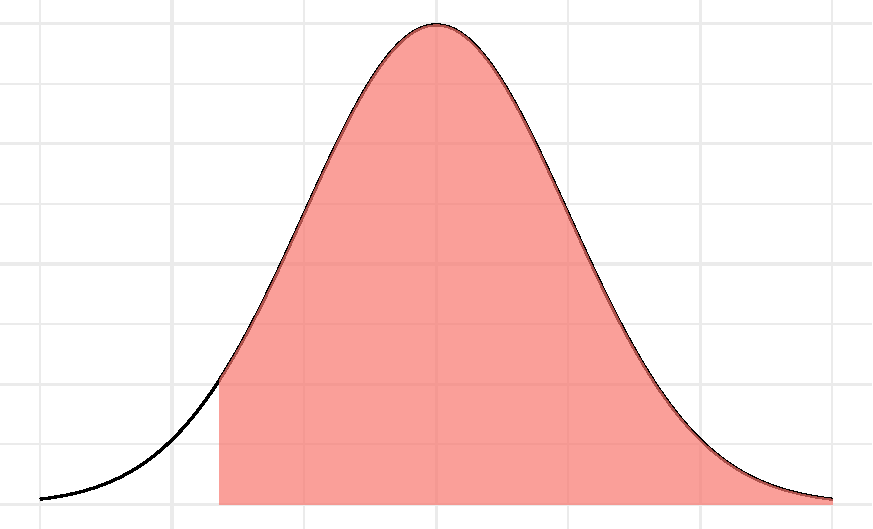
\includegraphics[width=0.7\linewidth]{/Users/younggeun/Documents/GitHub/nonparam-cvar/static/report/younggeunreport_files/figure-latex/lossdist-1} 

}

\caption{Loss Distribution - Can the financial institution still be in business after a catastrophic event?}\label{fig:lossdist}
\end{figure}

Why do economists care about this kind of measures? Both financial institutions and regulatory commitee should analyze the risk of their interesting portfolio. Tsay (\protect\hyperlink{ref-Tsay:2010aa}{2010}) interprets this in the two viewpoint. For financial institutions, VaR can be read as maximal loss of a financial position during a given time period for a given probability. It leads to meaning the measre of loss under normal market conditions. For regulartory committe, on the other hand, it can be read as minimal loss under extraordinary market circumstances.

As we can see in the Figure \ref{fig:lossdist}, VaR is defined using the probability distribution of loss. Let \(p\) be the right tail probability, the red area in the figure. Let \(l\) be the time horizon, let \(L(l)\) be the loss function of the asset from \(t\) to \(t + l\), and let \(F_l\) be the cdf of \(L(l)\). Then

\begin{equation}
  p = P \left[ L(l) \ge VaR \right]
  \label{eq:vardef}
\end{equation}

\begin{figure}[H]

{\centering 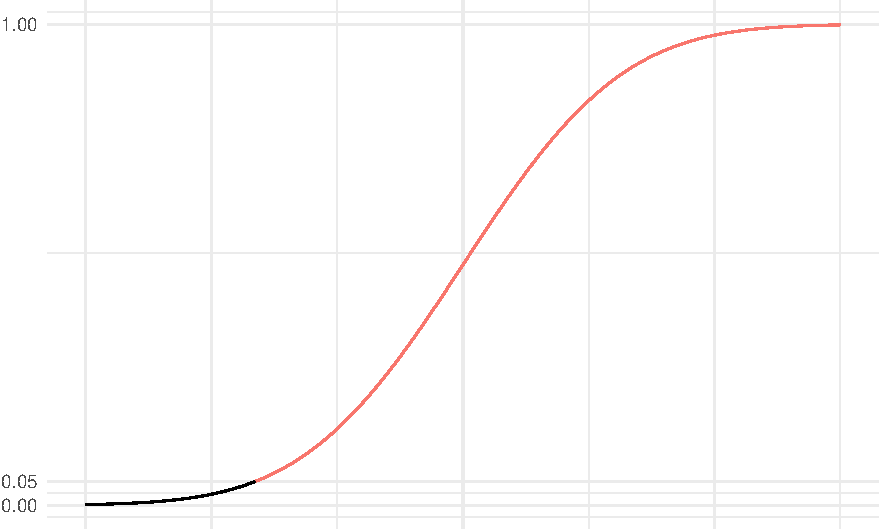
\includegraphics[width=0.7\linewidth]{/Users/younggeun/Documents/GitHub/nonparam-cvar/static/report/younggeunreport_files/figure-latex/lossquantile-1} 

}

\caption{CDF of Loss}\label{fig:lossquantile}
\end{figure}

See Figure \ref{fig:lossquantile}. VaR can be computed by finding the \(p\)-th quantile.

\begin{equation}
  VaR = \inf \left\{ x \mathpunct{:} F_l(x) \ge 1 - p \right\}
  \label{eq:varquant}
\end{equation}

\hypertarget{calculating-var}{%
\subsection{Calculating VaR}\label{calculating-var}}

There are many ways to get VaR in parametric way. Equation \eqref{eq:varquant} shows that VaR is the quantile in each time horizon. It is natural to employ quantile regression to get this quantile value.

This report consists of three parts. In Section \ref{background}, we covered basic concepts about CVaR and CES. In Section \ref{nonparam}, I reviewed the paper (Cai and Wang \protect\hyperlink{ref-cai:2008aa}{2008}) briefly. Theoretical parts were mostly skipped. In Section \ref{experiment}, we applied the method in both simulation setting and real data.

\hypertarget{background}{%
\section{Background}\label{background}}

\hypertarget{expected-shortfall}{%
\subsection{Expected Shortfall}\label{expected-shortfall}}

The reason why many authors only cover these two value-at-risk or expected shortfall that I will explain. Value at risk is famous and its concept is simple. In market, however, sometimes two portfolios can be merged. When this happens, the risk measure should not be greater than the sum of each. This is called subadditivity. VaR does not satistfy this property. It is possible for VaR to underestimate the actual loss. Expected loss is the one satisfying the condition. Expected shortfall is defined by the expected value of loss function if the VaR is exceeded.

\begin{equation}
  ES \mathpunct{:}=E \left[ L(l) \mid L(l) \ge VaR \right]
  \label{eq:esdef}
\end{equation}

In other words, while VaR cares the maximal loss in the right tail probability part, saying \(0.95\), ES cares average loss in the remaining part, \(0.05\).

\hypertarget{return}{%
\subsection{Return}\label{return}}

We prefer to use log return data. Let \(\{ P_t \}\) be the price series. Then the log return is defined by \(\{ Y_t \mathpunct{:}=\ln \frac{P_t}{P_{t - 1}} \}\). Loss occurs when the return \(\{ P_t - P_{t - 1} \}\) are negative, so we should use the negative returns or negative log returns.

Consider Taylor expansion for this log function. For any \(x_0 > 0\),

\begin{equation}
  \ln x \approx \ln x_0 + \frac{1}{x_0}(x - x_0)
\end{equation}

Write \(x = x_2\), \(x_0 = x_1\). Then

\begin{equation}
  \ln \frac{x_2}{x_1} \approx \frac{x_2}{x_1} - 1 = \frac{x_2 - x_1}{x_1}
  \label{eq:logpercent}
\end{equation}

Observe that the log return approximates to the change rate. Cai and Wang (\protect\hyperlink{ref-cai:2008aa}{2008}) used the following value in a real example part.

\[-100 Y_{t + 1} = -100 \ln \frac{P_{t + 1}}{P_t}\]

which approximates to percentage loss.

\hypertarget{conditional-information}{%
\subsection{Conditional Information}\label{conditional-information}}

In econometrics, conditional information are always researchers' interests. For example, we are interested in the exogenous variables like economic or market variables. When we look at return data, we can condition past observed returns.

Let \(\{ Y_t \}\) be stationary log returns and let \(\{ X_t \}\) be conditional information series.

\BeginKnitrBlock{definition}[Conditional Value-at-Risk]
\protect\hypertarget{def:condvar}{}{\label{def:condvar} \iffalse (Conditional Value-at-Risk) \fi{} }Let \(F(y \mid x)\) be the conditional cdf of \(Y_t\) given \(X_t = x\) and let \(S(y \mid x) \mathpunct{:}=1 - F(y \mid x)\). Then Conditional VaR is

\[\nu_p(x) \mathpunct{:}=S^{-1}(p \mid x)\]
\EndKnitrBlock{definition}

When formulating the conditional expected shortfall, we just add the term \(X_t = x\) in Equation \eqref{eq:esdef}. Let \(B \equiv \left\{ \omega \mathpunct{:} Y_t(\omega) \mid X_t = x \ge \nu_p(x) \right\} \in \mathcal{B}\). Then

\begin{equation}
  \begin{split}
    \mu_p(x) & = E \left[ Y_t \mid Y_t \ge \nu_p(x), X_t = x \right] \\
    & = \frac{1}{P(B)} \int_{B} Y_t dP \\
    & = \frac{1}{P\left( Y_t \ge \nu_p(x) \mid X_t = x \right)} \int_{\nu_p(x)}^\infty y f(y \mid x) dy \\
    & = \frac{1}{p} \int_{\nu_p(x)}^\infty y f(y \mid x) dy
  \end{split}
  \label{eq:cesformul}
\end{equation}

\hypertarget{nonparam}{%
\section{Nonparametric Estimation}\label{nonparam}}

The workflow of estimating is very simple. It uses the formulation of each CVaR and CES. Just put estimating notation in Equation \eqref{eq:cesformul}.

\begin{equation}
  \hat\mu_p(x) = \frac{1}{p} \int_{\hat\nu_p(x)}^\infty y \hat{f}(y \mid x) dy
  \label{eq:ceshat}
\end{equation}

Observe \(\hat\mu_p(x)\) and \(\hat{f}(y \mid x)\). After estimating these two, we will plug the above integration and get the result. THen we can summarize the prcess as follows.

\begin{enumerate}
\def\labelenumi{\arabic{enumi}.}
\tightlist
\item
  Estimate the conditional pdf \(\hat{f}(y \mid x)\).
\item
  Estimate the conditional cdf \(\hat{f}(y \mid x)\).
\item
  Invert the conditional cdf, and get \(\hat\nu_p(x)\).
\item
  Plugging, and get \(\hat\mu_p(x)\).
\end{enumerate}

\hypertarget{double-kernel-local-linear}{%
\subsection{Double Kernel Local Linear}\label{double-kernel-local-linear}}

Consider any symmetric kernel \(K_h(\cdot)\). Then by Taylor expansion,

\begin{equation}
  \begin{split}
    E [ K_{h_0}(y - Y_t) \mid X_t = x ] & = K_{h_0} \ast f_{y \mid x} (y) \\
    & = f(y \mid x) + \frac{h_0^2}{2} \mu_2(K) f^{(2)}(y \mid x) + o(h_0^2)
  \end{split}
  \label{eq:convolution}
\end{equation}

where \(\mu_j(K) = \int_{\mathbb{R}}u^j K(u) du\). Thus, we now have a smoothing problem

\begin{equation}
  f(y \mid x) \approx E \left[ K_{h_0}(y - Y_t) \mid X_t = x \right]
  \label{eq:smoothing}
\end{equation}

Different with the other usual smoothing setting, the response becomes \(Y_t^{\ast}(y) \equiv K_{h_0}(y - Y_t)\). Given this, implement local linear least squares.

\begin{equation}
  \hat{f}(y \mid x) = \mathop{\mathrm{argmin}}_{\alpha(x), \beta(x)} \sum_{t = 1}^n W_h (x - X_t) \left[ Y_t^{\ast}(y) - \alpha(x) - \beta(x) (X_t - x) \right]^2
  \label{eq:doublell}
\end{equation}

This is called double local linear in that the problem involves in the two kernel, \(K_{h_0}\) and \(W_h\). Recall that the local linear estimate is equivalent to the weighted least squares. Let \(\mathbf{Y}_y^{\ast} = \left( Y_1(y), \ldots, Y_n(y) \right)^T \in \mathbb{R}^n\), let \(\mathbf{b}_x(x_t) \mathpunct{:}=(1, x_t - x)^T \in \mathbb{R}^2\), let \(\mathbf{b}_x(x) = \mathbf{e}_1 \mathpunct{:}=(1, 0)^T\), let \(X_x \mathpunct{:}=\left( \mathbf{b}_x(x_i)^T \right) \in \mathbb{R}^{n \times 2}\), and let \(W_x \mathpunct{:}=diag(W_h(x - X_j)) \in \mathbb{R}^{n \times n}\). Then the local linear solution is given by \(\hat{f}_{ll} = \hat\alpha\),

\begin{equation}
  \begin{split}
    \hat{f}_{ll}(y \mid x) & = \mathbf{e}_1^T (X_x^T W_x X_x)^{-1} X_x^T W_x \mathbf{Y}_y^{\ast} \\
    & = \mathbf{l}(x)^T \mathbf{Y}_y^{\ast} \\
    & \equiv \sum_{t = 1}^n l_t(x) Y_t^{\ast}(y)
  \end{split}
  \label{eq:llsolution}
\end{equation}

Cai and Wang (\protect\hyperlink{ref-cai:2008aa}{2008}) provides the exact form of each element by matrix calculation in the paper. This linear form of pdf easily gives its cdf. This LL estimator has some good properties such as differentiability. The conditional cdf can be calculated by

\begin{equation}
  \begin{split}
    \hat{F}_{ll}(y \mid x) & = \int_\infty^y \hat{f}_{ll}(y \mid x) dy \\
    & = \sum_{t = 1}^n l_t(x) G_{h_0}(y - Y_t)
  \end{split}
  \label{eq:llcdf}
\end{equation}

where \(G(\cdot)\) is the cdf of \(K(\cdot)\). Since it is cdf, so it must be \(\hat{F}_{ll} \in [0, 1]\) and monotone increasing. Double local linear, however, does not guarantee these properties.

\hypertarget{weighted-nadaraya-watson}{%
\subsection{Weighted Nadaraya Watson}\label{weighted-nadaraya-watson}}

Since the above estimator cannot give a desirable cdf to us, we consider another method, weighted nadaraya watson suggested by Cai (\protect\hyperlink{ref-cai2001weighted}{2001}). The form is similar to the nadaraya watson estimator.

\begin{equation}
  \hat{F}_{NW}(y \mid x)  = \sum_{t = 1}^n W_{c, t}(x, \lambda) I(Y_t \le y)
  \label{eq:wnw}
\end{equation}

where the WNW weights given by

\begin{equation}
  W_{c,t}(x, h) = \frac{p_t(x) W_h (x - X_t)}{\sum\limits_{i = 1}^n p_i(x) W_h (x - X_i)}
  \label{eq:wnwkernel}
\end{equation}

The term ``weighted'' is due to the weight for each kernel. \(\{ p_t(x) \}\) is chosen by

\begin{equation}
  p_t(x) = \frac{1}{n \left[ 1 + \lambda(X_t - x) W_h (x - X_i) \right]} \ge 0
  \label{eq:wnwpt}
\end{equation}

We should find \(\lambda\) maximizing the empirical log likelihood function

\begin{equation}
  L_n(\lambda) = - \sum_{t = 1}^n \ln \left[ 1 + \lambda(X_t - x) W_h(x - X_i) \right]
  \label{eq:emplike}
\end{equation}

Cai (\protect\hyperlink{ref-cai2001weighted}{2001}) recommended employing Newton-Raphson to find it.

\hypertarget{weighted-double-kerenl-local-linear}{%
\subsection{Weighted Double Kerenl Local Linear}\label{weighted-double-kerenl-local-linear}}

Weighted Nadaraya Watson estimator for conditional cdf (Equation \eqref{eq:wnw}) can fill the defect of local linear (Equation \eqref{eq:llcdf}). In Equation \eqref{eq:llsolution}, Cai and Wang (\protect\hyperlink{ref-cai:2008aa}{2008}) can replace the linear smoother with WNW weights. This is called the weighted double kernel local linear estimator.

\begin{equation}
  \hat{f}_{cai}(y \mid x) = \sum_{t = 1}^n W_{c,t}(x, h) Y_t^{\ast}(y)
  \label{eq:wdkllpdf}
\end{equation}

It proceeds in a similar way that the the conditional cdf can be estimated by

\begin{equation}
  \hat{F}_{cai}(y \mid x) = \sum_{t = 1}^n W_{c,t}(x, h) G_{h_0}(y - Y_t)
  \label{eq:wdkllcdf}
\end{equation}

The next step is estimating \(\hat\nu_p(x)\) and \(\hat\mu_p(x)\) one by one. Let \(\hat{S}_{cai}(y \mid x) = 1 - \hat{F}_{cai}(y \mid x)\). By inverting this function, we can get the CVaR function.

\begin{equation}
  \hat\nu_p^{(cai)}(x) = \hat{S}_{cai}^{-1}(p \mid x)
  \label{eq:wdkllcvar}
\end{equation}

When inverting it, I used Equation \eqref{eq:varquant}. Finally, we plug \(\hat\nu_p(x)\) and \(\hat{f}_{cai}(y \mid x)\) into Equation \eqref{eq:ceshat}. Then

\begin{equation}
  \hat\mu_p(x) = \frac{1}{p} \sum_{t = 1}^n W_{c,t}(x, h) \left[ Y_t \bar{G}_{h_0} (\hat\nu_p(x) - Y_t) + h G_{1, h_0}(\hat\nu_p(x) - Y_t) \right]
  \label{eq:wdkllces}
\end{equation}

where \(\bar{G}(u) = 1 - G(u)\) and \(G_1(u) = \int_u^\infty v K(v) dv\).

\hypertarget{asymptotic-normality}{%
\subsection{Asymptotic Normality}\label{asymptotic-normality}}

Cai and Wang (\protect\hyperlink{ref-cai:2008aa}{2008}) has shown that each estimator follows Normal distribution at both interior and boundary point. Since the formulation is quite complicated, I provide Monte Carlo simulation setting here. Consider AR(1)-GARCH(0,1) model as in the paper.\footnote{Authors wrote that the model was ARCH(1), but many textbooks including Tsay (\protect\hyperlink{ref-Tsay:2010aa}{2010}) specify that model as GARCH(0,1).} This setting continues to the next simulation section.

\BeginKnitrBlock{example}[AR(1)-GARCH(0,1) Model]
\protect\hypertarget{exm:garch}{}{\label{exm:garch} \iffalse (AR(1)-GARCH(0,1) Model) \fi{} }With \(X_t = Y_{t - 1}\),

\[
\begin{cases}
  Y_t = 0.01 + 0.62 X_t + \sigma_t \epsilon_t \\
  \sigma_t^2 = 0.15 + 0.65 \sigma_{t - 1}^2 \\
  \epsilon_t \sim N(0, 1)
\end{cases}
\]
\EndKnitrBlock{example}

Monte Carlo Samples were generate by the following procedure.

\begin{enumerate}
\def\labelenumi{\arabic{enumi}.}
\tightlist
\item
  For fixed \(x\),
\item
  Generate GARCH(0, 1): \((\sigma_t, \epsilon_t)\)
\item
  Generate \(Y_t\) using AR(1) for each \(X_t = Y_{t - 1}\)
\item
  AR(1): \(Y_t = 0.01 + 0.62 Y_{t - 1} + \sigma_t \epsilon_t\)
\end{enumerate}

\hypertarget{interior}{%
\subsubsection{Interior}\label{interior}}

\begin{figure}[H]

{\centering 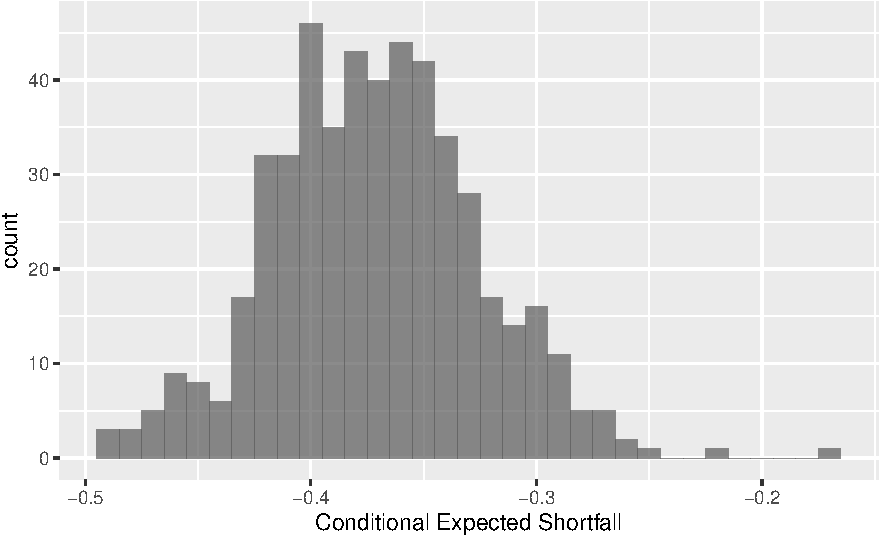
\includegraphics[width=0.7\linewidth]{/Users/younggeun/Documents/GitHub/nonparam-cvar/static/report/younggeunreport_files/figure-latex/wdkllnormal-1} 

}

\caption{Asymptotic normality for $\hat\mu_p(x)$ in interior point}\label{fig:wdkllnormal}
\end{figure}

In Figure \ref{fig:wdkllnormal}, we can see that \(\hat\mu_p(x)\) follows the normal distribution approximately at \(x = -0.734\).

\hypertarget{boundary}{%
\subsubsection{Boundary}\label{boundary}}

Cai and Wang (\protect\hyperlink{ref-cai:2008aa}{2008}) proved at the left boundary point \(x = ch\), \(0 < c < 1\).

\begin{figure}[H]

{\centering 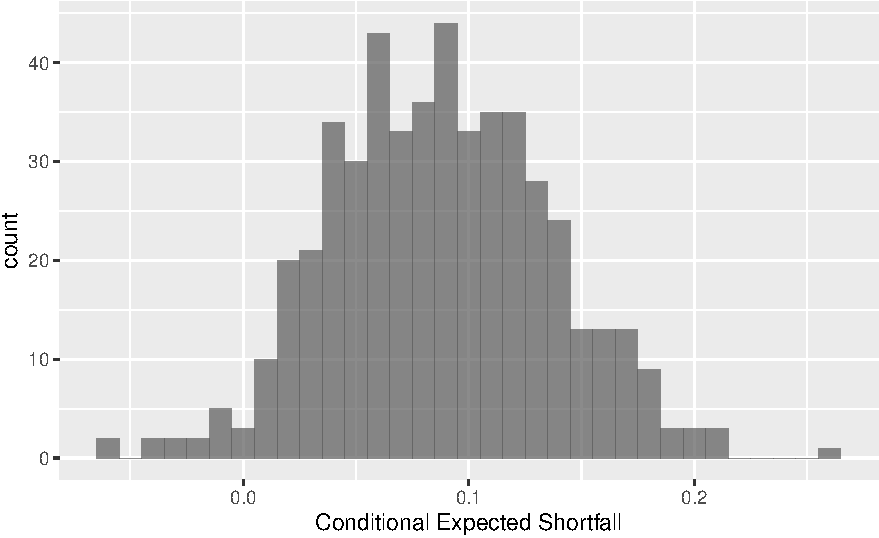
\includegraphics[width=0.7\linewidth]{/Users/younggeun/Documents/GitHub/nonparam-cvar/static/report/younggeunreport_files/figure-latex/wdkllboundary-1} 

}

\caption{Asymptotic normality for $\hat\mu_p(x)$ at left boundary}\label{fig:wdkllboundary}
\end{figure}

Similarly, Figure \ref{fig:wdkllboundary} presents asymptotic normality of WDKLL estimator of CES at the left boundary point.

\hypertarget{experiment}{%
\section{Experiments}\label{experiment}}

\hypertarget{simulation}{%
\subsection{Simulation}\label{simulation}}

Now we try another simulation under Example \ref{exm:garch}. This model implies the true CVaR and CES. Since \(\epsilon_t \sim N(0, 1)\),

\begin{equation}
  \sigma_t \epsilon_t \sim N(0, \sigma_t^2)
  \label{eq:garchterm}
\end{equation}

By construction,

\begin{equation}
  Y_t \mid X_t \sim N \left( 0.01 + 0.62 X_t, \sigma_t^2 \right)
  \label{eq:arterm}
\end{equation}

Given this conditional pdf, we can compute cdf using statistical package such as \href{https://www.r-project.org}{\texttt{R}}. The procedure after this is same with before. In this Monte Carlo simulation setting, we want to simulate the expected prediction error between the true \(\mu_p(x)\) and \(\hat\mu_p(x)\). Absolute loss was used following Cai and Wang (\protect\hyperlink{ref-cai:2008aa}{2008}). Figure \ref{fig:mctest} shows the structure of MC simulation. After training each model using each MC sample, we test it in the independent test set. Individual samples and a test set are generated as follows.

\begin{enumerate}
\def\labelenumi{\arabic{enumi}.}
\tightlist
\item
  For fixed \(x_t\) (pre-determined grid points)
\item
  Generate GARCH(0, 1): \((\sigma_t, \epsilon_t)\)
\item
  Generate \(Y_t\) using AR(1) for each \(X_t = Y_{t - 1}\)
\item
  AR(1): \(Y_t = 0.01 + 0.62 Y_{t - 1} + \sigma_t \epsilon_t\)
\end{enumerate}

\begin{figure}[H]

{\centering 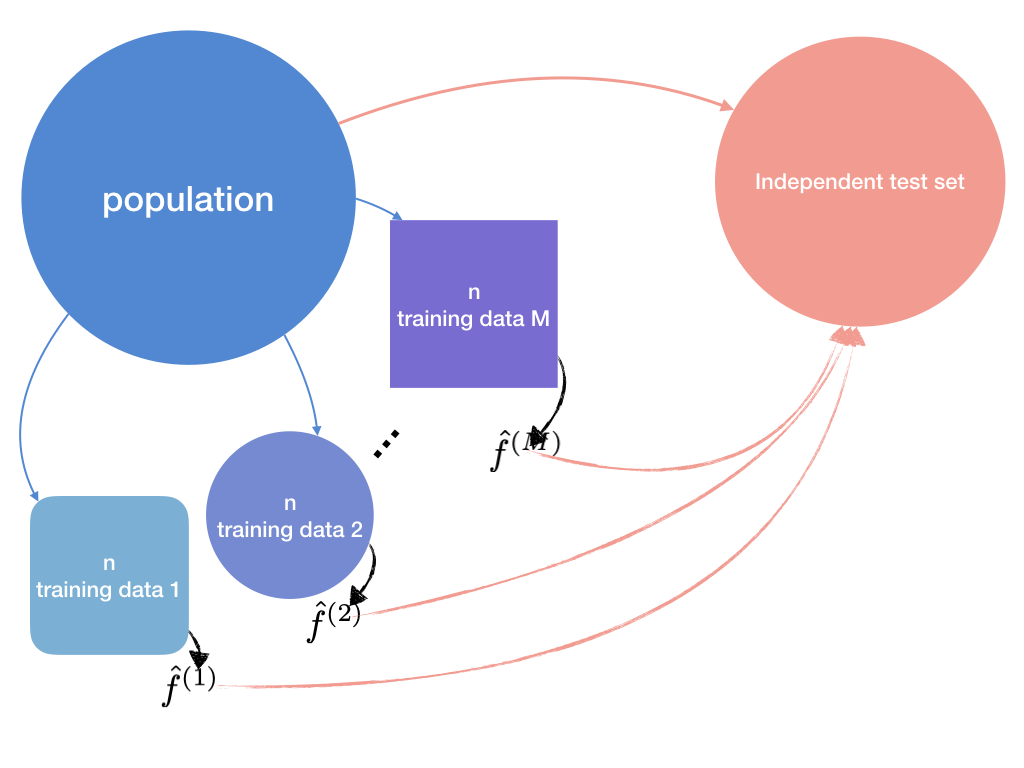
\includegraphics[width=0.7\linewidth]{../docs/mc_epe} 

}

\caption{Simulating Expected prediction error}\label{fig:mctest}
\end{figure}

See Figure \ref{fig:wdkllnw}. WDKLL estimator produces much less expected prediction error in each bandwidth than usual Nadaraya Watson estimator.

\begin{figure}[H]

{\centering 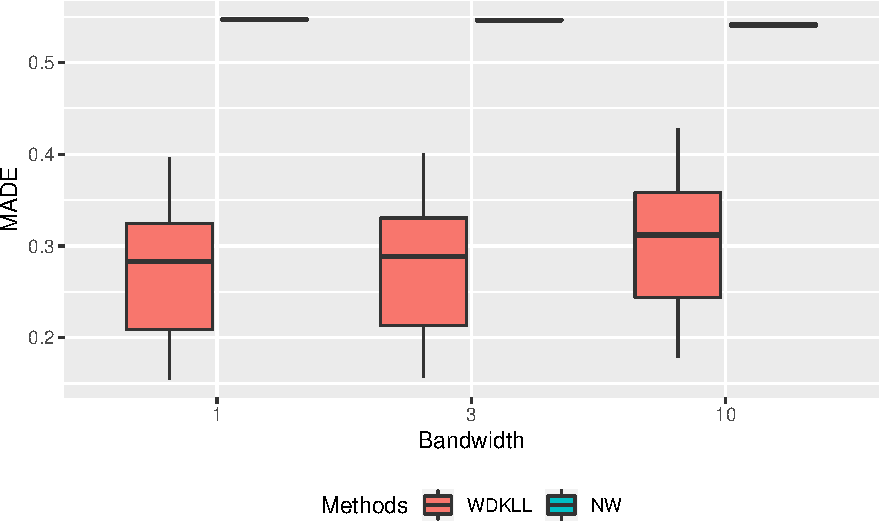
\includegraphics[width=0.7\linewidth]{/Users/younggeun/Documents/GitHub/nonparam-cvar/static/report/younggeunreport_files/figure-latex/wdkllnw-1} 

}

\caption{WDKLL versus Nadaraya-Watson}\label{fig:wdkllnw}
\end{figure}

\hypertarget{data-analysis}{%
\subsection{Data Analysis}\label{data-analysis}}

We can implement CVaR and CES to measure risk of Bitcoin. We analyze \(607\) daily prices of bitcoin from \(2018-04-05\) to \(2019-12-12\).

\begin{figure}[H]

{\centering 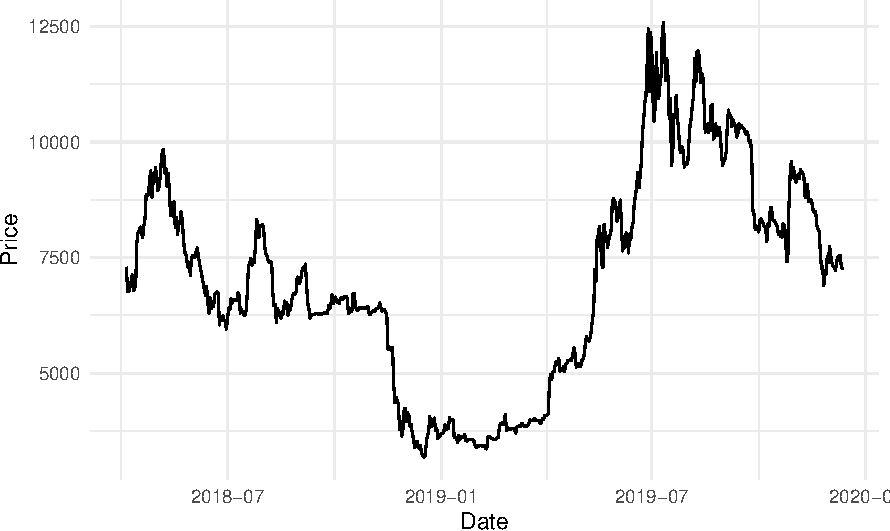
\includegraphics[width=0.7\linewidth]{/Users/younggeun/Documents/GitHub/nonparam-cvar/static/report/younggeunreport_files/figure-latex/bitprice-1} 

}

\caption{Bitcoin price in USD}\label{fig:bitprice}
\end{figure}

We use \(y_t \mathpunct{:}=- 100 \ln \frac{P_t}{P_{t - 1}}\) as daily return to approximate percentage loss.

\begin{figure}[H]

{\centering 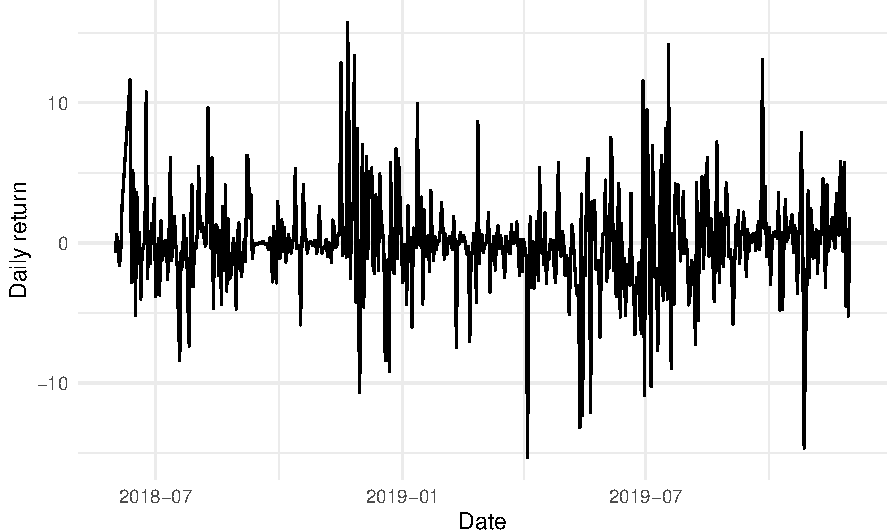
\includegraphics[width=0.7\linewidth]{/Users/younggeun/Documents/GitHub/nonparam-cvar/static/report/younggeunreport_files/figure-latex/bitreturn-1} 

}

\caption{Daily return of bitcoin price}\label{fig:bitreturn}
\end{figure}

Figure \ref{fig:bitreturn} is the daily return \(\{ y_t \}\). We now try to estimate using this \(y_t\) given the first lagged variable \(x_t = y_{t - 1}\).

Look at Figure \ref{fig:cvarcoin}. It is the plot of CVaR for each conditional information \(x_t = y_{t - 1}\). CVaR which is the maximal loss under \(0.95\) probability is increasing given the last day return. How about the other \(0.05\) case?

\begin{figure}[H]

{\centering 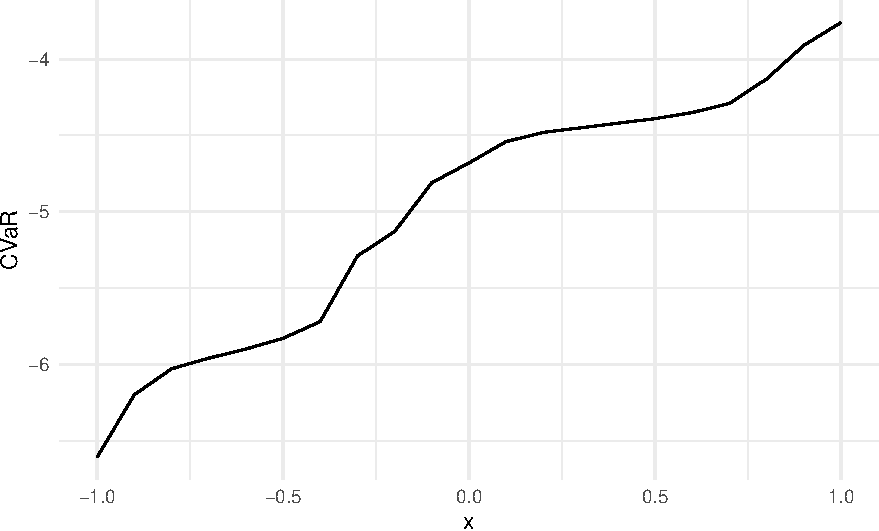
\includegraphics[width=0.7\linewidth]{/Users/younggeun/Documents/GitHub/nonparam-cvar/static/report/younggeunreport_files/figure-latex/cvarcoin-1} 

}

\caption{Conditional Value-at-Risk given each lagged variable value}\label{fig:cvarcoin}
\end{figure}

See Figure \ref{fig:cescoin}. This is the conditional expected shortfall. Recall that we are dealing with negative returns. Thus, positive \(x_t\) means the loss. We can expecte that its price is more likely to fall if there were a loss within the last day than if there was a same amount of positive return.\footnote{This interpretation have followed the one by Cai and Wang (\protect\hyperlink{ref-cai:2008aa}{2008})}

\begin{figure}[H]

{\centering 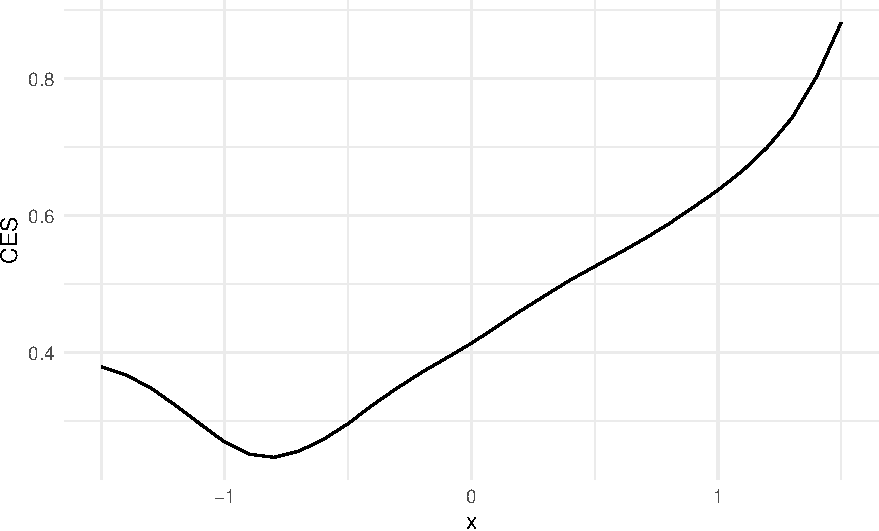
\includegraphics[width=0.7\linewidth]{/Users/younggeun/Documents/GitHub/nonparam-cvar/static/report/younggeunreport_files/figure-latex/cescoin-1} 

}

\caption{Conditional Expected Shortfall given each lagged variable value}\label{fig:cescoin}
\end{figure}

\hypertarget{conclusion}{%
\section{Conclusion}\label{conclusion}}

\hypertarget{discussion}{%
\subsection{Discussion}\label{discussion}}

\newpage

\hypertarget{references}{%
\section*{References}\label{references}}
\addcontentsline{toc}{section}{References}

\hypertarget{refs}{}
\begin{cslreferences}
\leavevmode\hypertarget{ref-cai2001weighted}{}%
Cai, Zongwu. 2001. ``Weighted Nadaraya--Watson Regression Estimation.'' \emph{Statistics \& Probability Letters} 51 (3): 307--18.

\leavevmode\hypertarget{ref-cai:2008aa}{}%
Cai, Zongwu, and Xian Wang. 2008. ``Nonparametric estimation of conditional VaR and expected shortfall.'' \emph{Journal of Econometrics} 147 (1): 120--30. \url{https://doi.org/10.1016/j.jeconom.2008.09.005}.

\leavevmode\hypertarget{ref-Tsay:2010aa}{}%
Tsay, Ruey S. 2010. \emph{Analysis of Financial Time Series}. John Wiley \& Sons.
\end{cslreferences}

\end{document}
